\chapter{Conflict Resolution}
\label{sec:conflicts}

Conflicts arise naturally in a participatory network, as \sys is
designed to allow multiple, distributed principals to author the network configuration.
For example, one principal may issue a request to deny traffic to
TCP port 80, while another may request  such traffic be allowed.
This chapter discusses how \sys handles conflicts between overlapping requests.

Two requests overlap when the interchapter of their
respective flowgroups is not empty, \ie, there are some flows that
match both.  As described in \xref{sec:overview}, principals
make requests in the context of a share, and accepted requests
become policy atoms residing in this share. Policy atoms, then,
inherit from the share tree a natural hierarchical relationship,
which we call the \emph{policy tree}. The network's effective policy is a function
of the set of all policy atoms, their position in the tree, and the
semantics of conflict resolution between overlapping policy atoms.

\begin{figure}
\centering
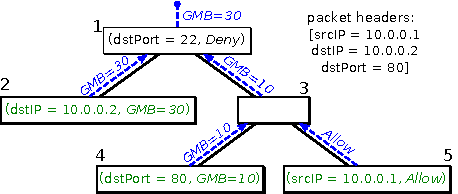
\includegraphics{figs/evaltree}
\caption{Evaluation of a single packet}
\label{f:evaltree}
\end{figure}

The semantics of the policy tree is the final action it produces on an
individual packet, after it has consolidated the actions of all
policy atoms in the tree. Figure~\ref{f:evaltree} illustrates a packet's
evaluation: matching policy atoms (shown in green) produce an action,
such as \priv{Allow} (shown in blue), and conflicts are resolved up the
hierarchy until a final action is emitted from the tree.

The policy tree is a declarative representation of the effective policy implemented by
\sys and installed in the physical network. In \sys, we represent
policy trees using HFTs, or Hierarchical Flow Tables~\cite{Ferguson:2012b}.
HFTs are a natural choice for \sys as they provide two key features:
first, flexible conflict resolution through the use of \emph{conflict resolution operators};
and second, a formally-verified compiler from HFTs to the flow match tables
used in OpenFlow.
We now describe how \sys uses the operators to resolve conflicts (\xref{sec:conflict-resolution-operators}),
the compiler to strictly or partially fulfill requests (\xref{sec:strict-partial}),
and the complexity of this approach (\xref{sec:compiler-complexity}).

\section{Conflict-resolution Operators}
\label{sec:conflict-resolution-operators}

%\begin{figure}[t]
%\begin{small}
%\fbox{$+_P : A \times A \rightarrow A$}
%\begin{displaymath}
%\begin{array}{lclcl}
%\textbf{Deny} & +_P & \textbf{Allow} & = & \textbf{Allow} \\
%\textbf{Allow} & +_P & \textbf{Allow} & = & \textbf{Allow} \\
%A_P & +_P & \textbf{Deny} & = & \textbf{Deny} \\
%\textbf{Deny} & +_P & \textbf{GMB}(n) & = & \textbf{GMB}(n) \\
%\textbf{GMB}(m) & +_P & \textbf{GMB}(n) & = & \textbf{GMB}(\max(m,n)) \\
%\textbf{GMB}(m) & +_P & \textbf{Allow} & = & \textbf{GMB}(m) \\
%\textbf{Allow} & +_P & \textbf{GMB}(m) & = & \textbf{GMB}(n)
%\end{array}
%\end{displaymath}
%
%\fbox{$+_S : A \times A \rightarrow A$}
%\begin{displaymath}
%\begin{array}{lclcl}
%\textbf{Deny} & +_S & A_2 & = & \textbf{Deny} \\
%\textbf{GMB}(m) & +_S & \textbf{GMB}(n) & = & \textbf{GMB}(\max(m,n)) \\
%\textbf{GMB}(m) & +_S & \textbf{Allow} & = & \textbf{GMB}(m) \\
%\end{array}
%\end{displaymath}
%\end{small}
%{\small The $+_S$ operator is commutative. We only show representative cases.}
%
%\caption{\sys's conflict-resolution operators}
%\label{f:paneconflicts}
%
%\end{figure}



HFTs resolve conflicts through the use of conflict resolution operators.
These operators take two conflicting requests as input, and return a single
resolved request. For example, a packet which matches policy atoms from \priv{Reserve}(10)
and \priv{Reserve}(30) may be resolved to the higher guaranteed bandwidth,
\priv{Reserve}(30), as occurs at Node 1 in Figure~\ref{f:evaltree}.

HFTs have three types of conflict-resolution operators at each node in the tree. 
These multiple types allow HFTs to resolve different types of conflicts using
independent logic: $+_D$ is used to resolve conflicts between requests
within the same share, $+_P$ between conflicting requests in parent and
child shares, and $+_S$ to resolve conflicts between sibling shares.
Their placement directly in the nodes allows conflict resolution to make implicit use of
the hierarchy.
This design makes it simple to express intuitive conflict resolutions such as
``child overrides parent.''
%Therefore, the choice of conflict-resolution operators is a key policy decision.

%The \treelang design allows for complex
%conflict-resolution operators, and could support different operators at
%each node in the tree.
%However, 
For \sys we chose simple conflict-resolution operators in the
interest of user and administrator understanding.
%Figure~\ref{f:sysconflicts} specifies \sys's conflict-resolution
%operators. {\color{red}(What about other resources??)}
\sys's parent-child operator ($+_P$) specifies a ``child
overrides parent'' policy for admission control. \sys's $+_S$ and $+_D$
operators are identical, and specify a ``\priv{Deny} overrides
\priv{Allow} policy'' between siblings.

%\remark{\color{red} Say that conflict resolution operators can break hints?}

%These operators' simple design is heavily influenced by \sys's
%first come-first serve approach to granting requests -- for example,
%the operators do not consider the principal who made the request;
%each request is treated equally within its hierarchical context.
%However, by taking advantage of this design flexibility, operators
%which resolve conflicts by using priorities could be introduced.
%Because such an approach would lead to previously accepted requests
%being preempted, the \sys controller would need to maintain a
%connection to each principal to provide preemption notifications.
%Avoiding this complexity is an additional benefit of \sys's current,
%simple approach.

\section{Strict vs Partial Fulfillment}
\label{sec:strict-partial}

We now return to \sys's \emph{strict} and \emph{partial} modes of
fulfillment, first introduced with the \priv{Allow} and \priv{Deny}
privileges. In each mode, a request is first authenticated against the
share tree, then, as shown in Figure~\ref{f:system}, \sys verifies the resulting policy tree can be
compiled to a valid network configuration.
After this verification, the two modes differ.

In strict mode, \sys ensures that a request's specified action
is the same as the action returned by HFT's \emph{eval}
function for all packets in the request's flowgroup -- that is, no
conflict resolution operator has changed the resulting action for
any matching packets.
More formally, when a request with match rule $M$ and action
$A$ is added to a policy tree, yielding tree $T$,
$\forall\ \mathrm{packets}\ K \in \{ K | M \cap K \ne \emptyset \}, \mathit{eval} (T, K) = A$.
If this condition does not hold, the request is rejected.
In partial mode, the request is not subject to this check, and may
even be relaxed -- for example, a request for 30 Mbps of guaranteed
bandwidth on a share with only 20 Mbps available will be relaxed
to a request for 20 Mbps. 

These modes are useful for three reasons. First, strict mode provides
the principal with a guarantee that the request will be implemented
in the network as specified. This is a limited form of change-impact
analysis: \emph{was the impact of my change on the network's configuration
what I expected? If not, cancel the request.} We will expand
\sys's ability to provide change-impact analysis in future work.

Second, partial mode improves support
for concurrent requests, as at least a relaxed form of a partial request will succeed.
Without this, a principal faces the risk of repeatedly crafting
strict requests based on the network state at time $t_0$, only to have
the request arrive at time $t_2 > t_0$ and conflict with a request
accepted at time $t_1$, where $t_2 > t_1 > t_0$.

Finally, partial mode's ability to relax a request is a useful convenience.
For example, if a principal has permissions which affect dozens of
specific TCP ports in the range 1000-2000, yet not all of them, partial
requests can be made for that range, and the requests would be relaxed to
just the specific ports, freeing the principal from needing to specify the
particular ports on each request.

Partial reservations, such as the 20 Mbps received of the 30 Mbps requested
in the example above, are particularly useful as
applications can use them to provide upper-bounds for transfer time. Although the
faster reservation may have been preferred, the slower one still provides
predictability to the end-user (and in either scenario, the actual bandwidth
received by the transfer may be even higher than the guaranteed minimum).
Such a use case is different from that for bandwidth hints; with hints, the
principal does not know how the information will be used, if at all.

\begin{comment}
Can discuss why partial reservations make sense -- operations such as a
data backup can get a guarantee from the network, which allows them to
provide a predictable experience for the user. however, they don't need to
get a guarantee as high as the one they requested. this is different from a
hint situation in which the network control-plane understands more about
the traffic, say, that it will be predictable (information it can feed to
something like Theo's MicroTE) or that it will be a large flow, so that the
controller can proactively split elephant flows across redundant links.
\end{comment}

\section{Compiler Complexity}
\label{sec:compiler-complexity}

To realize a policy tree in OpenFlow hardware, we have to compile it
to flow tables for each switch. We use a variation of
Hierarchical Flow Tables (HFT)~\cite{Ferguson:2012b}. A direct
implementation of the HFT algorithm produces flow tables of size
$O(2^n)$, where $n$ is the size of the policy tree. The earlier
algorithm is therefore useless on all but trivial policies.  However,
we make two changes that greatly reduce the complexity:
the modified algorithm yields flow tables
of size $O(n^2)$ in $O(n^2)$ time. This section is an overview of our
results. 

OpenFlow flow tables are simple linear
sequences of patterns and actions. A flow can match several,
overlapping policy atoms in a policy tree and trigger
conflict-resolution that combines their policies. However, in an
OpenFlow flow table, a flow will only trigger the action of the
highest-priority matching pattern.

For example, suppose the policy tree has two atoms with the following
flowgroups:
\[
\begin{array}{l}
\paneshare{X}{Y}{\texttt{tcp}}{\star}{\star} \\
\paneshare{\star}{\star}{\texttt{tcp}}{\star}{\texttt{80}}
\end{array}
\]
Suppose flows that match the first flowgroup -- all flows from $X$ to
$Y$ -- are waypointed through some switch, and that flows that match
the second flowgroup -- all HTTP requests -- are given some bandwidth
reservation.  These two flowgroups overlap, thus a flow may be (1)
waypointed with a reservation, (2) only waypointed, (3) only given a
reservation, or (4) not be affected by the policy.

An OpenFlow flow table that realizes the above two-atom policy tree must have
entries for all four cases.  The original algorithm~\cite{Ferguson:2012b}
generates all possible combinations given trees of size $n$ --- \ie flow tables
of size $O(2^n)$.

We make two changes to prune the generated flow table: (1) we remove
all rules that generate empty patterns and (2) we remove all rules
whose patterns are fully shadowed by higher-priority rules. The
earlier algorithm is recursive, and we prune after each recursive
call.  It is obvious that this simple pruning does not affect the
semantics of flow tables. However, a surprising result is that it
dramatically improves the complexity of the algorithm.

The intuition behind our proof is that for sufficiently large policy trees,
the intersections are guaranteed to produce
duplicate and empty patterns that get pruned. To see this,
note OpenFlow patterns have a bit-vector that determines which fields
are wildcards.  Suppose two patterns have identical wildcard bits and
we calculate their intersection:

First, if the two patterns are identical, then so is their
  intersection. Of these three identical patterns, two get pruned.
Second, if the two patterns are distinct, since their wildcards are
  identical, they exactly match some field differently. Thus, their
  intersection is empty and pruned.

If patterns have $h$ header fields, there are only $2^h$ unique
wildcard bit-vectors. Therefore, if a policy tree has more than $2^h$
policy atoms, it is assured that some intersections create empty or duplicate
patterns that are pruned.

Our full complexity analysis shows that when the
number of policy atoms, $n$, is larger than $2^h$, then the
compilation algorithm runs in $O(n^2)$ time and produces a flow table
of size $O(n^2)$. OpenFlow 1.0 patterns are $12$-tuple, and our current
policies
only use $5$ header fields. Therefore, on policies
with more than $2^5$ policy atoms, the algorithm is quadratic.

\tightparagraph{Updating Flow Tables}

It is not enough for \sys to generate flow tables quickly. It must
also propagate switch updates quickly, as the time required to update
the network affects the effective duration of requests.
The OpenFlow protocol only allows switches to be updated one rule at a
time.  A naive strategy is to first delete all old rules, and then
install new rules. In \sys, we implement a faster strategy: the
controller state stores the rules deployed on each switch; to install
new rules, it calculates a ``diff'' between the new and old
rules. These diffs are typically small, since rule-table updates occur
when a subset of policy atoms are realized or unrealized.



